\documentclass[aps,prx,reprint,amsmath,amssymb,floatfix,nofootinbib,superscriptaddress]{revtex4-2}

\usepackage{graphicx}
\usepackage{dcolumn}
\usepackage{bm}
\usepackage{hyperref}
\usepackage{booktabs}
\usepackage{array}
\usepackage{xcolor}

\hypersetup{
  colorlinks=true,
  linkcolor=blue!50!black,
  citecolor=blue!50!black,
  urlcolor=blue!50!black,
  pdftitle={Leggett-Garg K3 Values Above 1 in Fibonacci-Anyon Braiding: 99.998\% of the Lueders Bound, and Exactly 1 for Ising Braiding},
  pdfauthor={Berkay Y{\"u}ksel Sayim},
  pdfsubject={quant-ph; Fibonacci anyons; Leggett-Garg inequality; macrorealism},
  pdfkeywords={Leggett-Garg inequality, Fibonacci anyons, non-Abelian braiding,
               macrorealism, Luders bound, topological quantum computation,
               modular tensor category, universality}
}

\begin{document}
\setcounter{secnumdepth}{3} % v1.2 series convention (1a/1b/2 consistency)

\title{Leggett--Garg $K_{3}$ Values Above 1 in Fibonacci-Anyon Braiding:\\
$99.998\%$ of the L\"uders Bound, and Exactly 1 for Ising Braiding}

\author{Berkay Y\"uksel Sayim}
\email{berksa@tutamail.com}
\affiliation{Independent Research, Germany\\
\href{https://orcid.org/0009-0004-4993-7352}{ORCID: 0009-0004-4993-7352}}

\date{2026-10-03}

\begin{abstract}
We numerically test the three-time Leggett--Garg inequality
$K_{3} \leq 1$ for the standard B$_{3}$ Fibonacci-anyon braiding
representation on the two-dimensional fusion space of three $\tau$ anyons.
Exhaustive enumeration over all $4^{L}$ braid words up to length $L=11$
and random sampling to $L=40$ show that $K_{3}$ saturates the L\"uders
bound $3/2$ to $99.998\%$, with the first violation already at $L=3$.
Two structural signatures accompany the saturation. First, replacing
the Fibonacci generators by the Ising-anyon generators on the same
$2$D fusion space gives $K_{3}=1$ exactly for every $L\leq11$ in the
exhaustive search and every random word tested at even
$L\in\{12,14,\ldots,40\}$---a sharp split that mirrors the Howard--Vala
no-Bell-violation result for Ising braiding in the spatial CHSH setting.
Second, an algebraic phase-deformation parameter $\delta$ tunes
a singular point
$\delta = 3\pi/5$ at which the generator $\sigma_{1}$ collapses to a
scalar to machine precision, so that every braid word reduces to a
global phase. The Fourier-period analysis of the $\delta$ dependence
reported in earlier versions of this letter is withdrawn. As a
consistency check, we confirm that
$K_{3}$ for the optimal $L=11$ word is initial-state independent
(every pure state and the maximally mixed state agree to
$\sim 10^{-15}$, machine precision),
as required by a generic $d=2$ trace identity for qubit observables.
All Yang--Baxter, unitarity, and $(\sigma_{1}\sigma_{2})^{3}$-scalar
sanity checks pass at machine precision for the undeformed generators
($\delta = 0$). The closest previously published work we identified,
``Leggett--Garg on a topological system,'' is
G\'omez-Ruiz \emph{et al.} (2018), which differs in three ways: the
system is abelian (Kitaev chain, not Fibonacci); the qubit basis is
formed by paired edge Majorana modes rather than the fusion channel
of three anyons; and $K_{3}$ is used as a probe of a topological
phase transition rather than as a saturation test. Code,
seeds, and data are released with the preprint.
\end{abstract}

\maketitle

\section{Introduction}

The Bell inequalities probe whether spatially separated subsystems can
be described by a joint local-realistic distribution; the
Leggett--Garg inequalities~\cite{LeggettGarg1985} probe the temporal
analogue---whether a single system carries a definite value of an
observable between measurements, independent of whether it is measured
(``macrorealism''), and under what conditions quantum mechanics can
violate it~\cite{KoflerBrukner2008}. For three projective measurements of a dichotomic
observable $Q \in \{+1,-1\}$ at times $t_{1} < t_{2} < t_{3}$, with
two-time correlators $C_{ij} \equiv \langle Q(t_{i})\,Q(t_{j}) \rangle$,
the simplest combination
\begin{equation}
  K_{3} \;=\; C_{12} + C_{23} - C_{13}
\end{equation}
satisfies $K_{3} \leq 1$ under macrorealism, $K_{3} \leq 3/2$ under
L\"uders projective quantum measurement on a two-level system (the
``temporal Tsirelson bound''~\cite{Budroni2014}), and $K_{3} \leq 3$
algebraically.

Non-Abelian anyons are the natural laboratory for asking whether a
\emph{topological} two-level system---a fusion-channel qubit whose
algebra has no tensor-product factorization into spatial
subsystems~\cite{NayakSimonStern2008}---also saturates the L\"uders
bound. The Fibonacci anyon model is the smallest model in which
braiding alone is computationally universal (dense in $\mathrm{SU}(2)$
on the relevant fusion space), while the Ising model, including its
Majorana-zero-mode realizations, gives only the Clifford group and is
provably unable to violate the spatial CHSH inequality when only
topologically protected stabilizer operations are
performed~\cite{HowardVala2012}; Clarke, Sau, and
Das~Sarma supply a non-Clifford phase gate for Majorana
wires~\cite{ClarkeSauDasSarma2016}. The two models
therefore form a natural \emph{universality split}: a property that
requires arbitrarily close approximation of generic unitaries should
discriminate sharply between them.

The temporal counterpart has not, to our knowledge, been measured. The closest published work we identified, ``Leggett--Garg on a topological system,'' is G\'omez-Ruiz
\emph{et al.}~\cite{GomezRuiz2018}, who tested $K_{3}$ for Dirac
qubits formed from edge Majorana modes of the abelian Kitaev chain.
We state up front how the present work differs, because this
demarcation defines the novelty claim:

\begin{center}\footnotesize
\setlength{\tabcolsep}{4pt}
\begin{tabular}{lll}
\toprule
                 & G\'omez-Ruiz 2018~\cite{GomezRuiz2018} & this work \\
\midrule
anyon type       & abelian            & \textbf{non-Abelian} \\
qubit basis      & edge Majoranas     & \textbf{$3\tau$ channel} \\
braiding         & none; platform Clifford-only & \textbf{universal} \\
role of $K_{3}$  & transition probe   & \textbf{saturation test} \\
saturation       & none reported      & \textbf{$99.998\%$ of $3/2$} \\
\bottomrule
\end{tabular}
\end{center}

\noindent The two papers are methodologically and physically distinct
sub-cases of ``Leggett--Garg on a topological system''. Apart from Brennen \emph{et al.}~\cite{Brennen2009}, who construct explicit CHSH-violating settings on the Fibonacci/Ising fusion spaces but do not test the temporal inequality, we identified no further Bell or Leggett--Garg work for Fibonacci or Ising anyons. Recent
solid-state and quantum processor demonstrations of non-Abelian
topological order~\cite{Andersen2023,Iqbal2024,Xu2024,Minev2025}
provide a plausible target for an experimental test but have, to our
knowledge, not yet been used for one.

We present the simplest possible numerical setup for the temporal
question. Section~\ref{sec:setup} fixes the generators, correlator,
and sanity checks. Section~\ref{sec:results} reports three connected
findings: (i)~Fibonacci L\"uders saturation to $99.998\%$; (ii)~an exact
$K_{3}=1$ for Ising at every length tested; (iii)~an algebraic
scalar-singularity point $\delta = 3\pi/5$. The subsection on the
$\delta$ dependence (Sec.~\ref{sec:sector-fourier}) withdraws the
Fourier-period analysis reported in earlier versions, and a consistency
check closes Section~\ref{sec:results}: the optimal $K_{3}$ does not
depend on the initial state.
Section~\ref{sec:discussion} relates the universality split to the
known CHSH split and lists what the results do \emph{not} say.

\section{Setup}
\label{sec:setup}

\subsection{Fusion space and observable}

We work on the two-dimensional fusion space of three $\tau$ anyons
with total charge $\tau$ in the Fibonacci modular tensor
category~\cite{NayakSimonStern2008}, identified with the standard
B$_{3}$ Burau-Jones representation. The dichotomic observable
$Q = \sigma_{z}$ corresponds to a measurement of the topological
charge of an anyon pair~\cite{Bonderson2008}; experimentally this is
the interferometric fusion outcome of the pair.

\subsection{Generators}

We use the standard Fibonacci $F$- and $R$-symbols~\cite{NayakSimonStern2008}:
\begin{equation}
  F \;=\;
  \begin{pmatrix} 1/\varphi & 1/\sqrt{\varphi} \\
                  1/\sqrt{\varphi} & -1/\varphi \end{pmatrix},
  \quad
  R_{1} = e^{-4\pi i/5},\ \ R_{\tau} = e^{+3\pi i/5},
\end{equation}
with $\varphi = (1+\sqrt{5})/2$, giving
\begin{equation}
  \sigma_{1} \;=\; \mathrm{diag}(R_{1},\,R_{\tau}\,e^{i\delta}),
  \qquad
  \sigma_{2} \;=\; F\,\sigma_{1}\,F.
\end{equation}
Here $\delta$ is an algebraic phase-deformation parameter: $\delta=0$
recovers the standard Fibonacci theory. For generic $\delta \neq 0$ the
deformed generators do not satisfy the braid (Yang--Baxter) relation
$\sigma_{1}\sigma_{2}\sigma_{1} = \sigma_{2}\sigma_{1}\sigma_{2}$, not
even up to a global phase. In $[0, 2\pi)$ it holds only at $\delta = 0$,
at $\delta = 3\pi/5$, where $\sigma_{1}$ and $\sigma_{2}$ become
multiples of the identity (Sec.~\ref{sec:singularity}), and at $\delta =
6\pi/5$, where they equal the complex conjugates of the $\delta = 0$
generators up to a global phase; all three points lie on the $240$-point
grid used below. The braid alphabet is
$\{\sigma_{1},\sigma_{1}^{-1},\sigma_{2},\sigma_{2}^{-1}\}$.

The Ising data~\cite{NayakSimonStern2008} on the analogous $2$D
fusion space are
\begin{equation}
  F_{\mathrm{I}} \;=\; \tfrac{1}{\sqrt{2}}
  \begin{pmatrix} 1 & 1 \\ 1 & -1 \end{pmatrix},
  \qquad
  R^{\sigma\sigma}_{1} = e^{-i\pi/8},
  \quad
  R^{\sigma\sigma}_{\psi} = e^{+i 3\pi/8},
\end{equation}
with $\sigma_{1},\sigma_{2}$ constructed identically; this is the
nonuniversal Clifford branch.

\subsection{Correlator}

For projective L\"uders measurement of $Q=\sigma_{z}$ at every time
step and any initial state, the two-time correlator separating two
measurements by a unitary $U$ is
\begin{equation}
  C(U) \;=\; \tfrac{1}{2}\,\mathrm{Re}\,\mathrm{Tr}\bigl[Z\,U\,Z\,U^{\dagger}\bigr],
\label{eq:correlator}
\end{equation}
with $Z=\sigma_{z}$. With equal-time braids $B$ between $t_{1}$--$t_{2}$
and $t_{2}$--$t_{3}$, so $U_{13}=B^{2}$, we have
\begin{equation}
  K_{3} \;=\; 2\,C(B) \,-\, C(B^{2}).
\end{equation}
The correlator~(\ref{eq:correlator}) is invariant under any global
phase of $U$, so we may use the full unitary generators without
projecting onto $\mathrm{SU}(2)$. This closed-form expression of the
correlator in terms of the connecting unitary follows the same
general treatment as the temporal-CHSH correlator of
Ref.~\cite{Fritz2010}.

\subsection{Sanity}

Before reporting results we verify generator consistency at $\delta =
0$. All checks
pass at machine precision:
\begin{center}\small
\begin{tabular}{lcc}
\toprule
& Fibonacci & Ising \\
\midrule
$\|\sigma_{i}\sigma_{i}^{\dagger}-I\|$ & $1.5\times10^{-16}$ & $5.6\times10^{-16}$ \\
$\|\sigma_{1}\sigma_{2}\sigma_{1}-\sigma_{2}\sigma_{1}\sigma_{2}\|$
                                      & $2.4\times10^{-16}$ & $2.8\times10^{-16}$ \\
$(\sigma_{1}\sigma_{2})^{3}$ scalar?  & yes, phase $e^{2\pi i/5}$
                                      & yes, phase $e^{-i\pi/4}$ \\
$\|(\sigma_{1}\sigma_{2})^{3}-\omega I\|$
                                      & $2.0\times10^{-16}$ & $2.5\times10^{-16}$ \\
\bottomrule
\end{tabular}
\end{center}
The central scalar of B$_{3}$ for Fibonacci is the fifth root of unity
$e^{2\pi i/5}$ (consistent with the conformal weight
$h_{\tau} = 2/5$~\cite{NayakSimonStern2008}); for Ising it is
$e^{-i\pi/4}$ (consistent with central charge $c=1/2$).

\subsection{Search}

For each $L \in \{1,\ldots,11\}$ we enumerate all $4^{L}$ braid words
and record the largest $K_{3}$. For $L \in \{12,\ldots,40\}$ we draw
$4\times 10^{5}$ uniformly random words per $L$. The deformation sweep
samples $\delta \in [0, 2\pi)$ at $240$ points, using exhaustive
$L \leq 9$ at each $\delta$. All computations use
\texttt{numpy} only; the random seed is fixed (see code release).

\section{Results}
\label{sec:results}

\begin{table*}
\caption{Best $K_{3}$ versus braid-word length $L$ for the Fibonacci
and Ising representations at $\delta=0$. Exhaustive search up to
$L=11$. The Fibonacci values approach the L\"uders bound $3/2$
already at $L=9$ (exhaustive maximum $99.984\%$; deeper random
sampling at $L\ge 22$ reaches $99.998\%$, never exactly; see
Sec.~\ref{sec:results}); the Ising values do not violate macrorealism
for any tested $L$.}
\label{tab:K3_L}
\centering
\begin{tabular}{rrcccc}
\toprule
$L$ & $\#$ words & $K_{3}^{(\mathrm{Fib})}$ & $C(B)^{(\mathrm{Fib})}$
    & $C(B^{2})^{(\mathrm{Fib})}$ & $K_{3}^{(\mathrm{Ising})}$ \\
\midrule
1  & 4         & 1.00000 &  1.0000 &  1.0000 & 1.00000 \\
2  & 16        & 1.00000 &  1.0000 &  1.0000 & 1.00000 \\
3  & 64        & 1.29180 &  0.8197 &  0.3475 & 1.00000 \\
4  & 256       & 1.40325 &  0.3475 & $-0.7082$ & 1.00000 \\
5  & 1\,024    & 1.29180 &  0.8197 &  0.3475 & 1.00000 \\
6  & 4\,096    & 1.47744 &  0.5704 & $-0.3366$ & 1.00000 \\
7  & 16\,384   & 1.43396 &  0.3212 & $-0.7915$ & 1.00000 \\
8  & 65\,536   & 1.47744 &  0.5704 & $-0.3366$ & 1.00000 \\
9  & 262\,144  & 1.49976 &  0.4977 & $-0.5043$ & 1.00000 \\
10 & 1\,048\,576 & 1.49783 & 0.4977 & $-0.5024$ & 1.00000 \\
11 & 4\,194\,304 & 1.49976 & 0.4977 & $-0.5043$ & 1.00000 \\
\bottomrule
\end{tabular}
\end{table*}

\subsection{Fibonacci: $K_{3}$ up to $99.998\%$ of the L\"uders bound}

Table~\ref{tab:K3_L} lists the best $K_{3}$ for every $L \leq 11$.
The first violation of macrorealism occurs already at $L=3$, with
$K_{3} = 1.292$. The maximum over exhaustive search is
$K_{3}^{\max} = 1.499762$ at $L=11$ (tied with $L=9$), attained by the word
$\sigma_{1}\sigma_{2}^{2}\sigma_{1}^{-3}\sigma_{2}^{2}\sigma_{1}^{-1}\sigma_{2}\sigma_{1}$
(correcting a mistranscribed 14-letter word reported in v1.0--v1.1;
the corrected 11-letter word is the one recorded by the deposited
search code, \texttt{lgi\_fibonacci.py}, and independently
re-verified by two algorithmically distinct enumeration routes) and
by $351$ other equivalent words (352 in total tie the maximum to
machine precision); the gap to the L\"uders bound is
$2.4\times 10^{-4}$. Random sampling at $L \geq 22$ yields
$K_{3} = 1.499964$, a gap of $3.6\times 10^{-5}$, i.e.\ $99.998\%$ of
the L\"uders bound. We never observe a violation of the L\"uders
bound, consistent with the structural impossibility for three
projective measurements of a two-level system.

A characteristic nonmonotonicity in the best-at-exactly-$L$ curve
appears at $L = 5,7,10$, visible in Fig.~\ref{fig:main}(a). This is the
expected fingerprint of a discrete dense group: the word set at
length $L+1$ is constructed afresh and need not contain the best
length-$L$ word, so the per-length maximum can decrease.
No simple length-divisibility rule governs which $L$ attains the
saturating value: Table~\ref{tab:K3_L} shows $L=9$ and $L=11$ tied at
the maximum $K_{3}=1.499762$, while $L=6$, a central-element length
$(\sigma_{1}\sigma_{2})^{3k}$ with $k=1$, reaches only $K_{3}=1.47744$,
well below the $L=9/11$ value (an earlier conjecture that lengths
divisible by $6$ are structurally favored is not supported by the
data and is retracted here). The reverse-monotonic version
``best at length $\leq L$'' is monotone by construction.

\begin{figure*}[t]
\centering
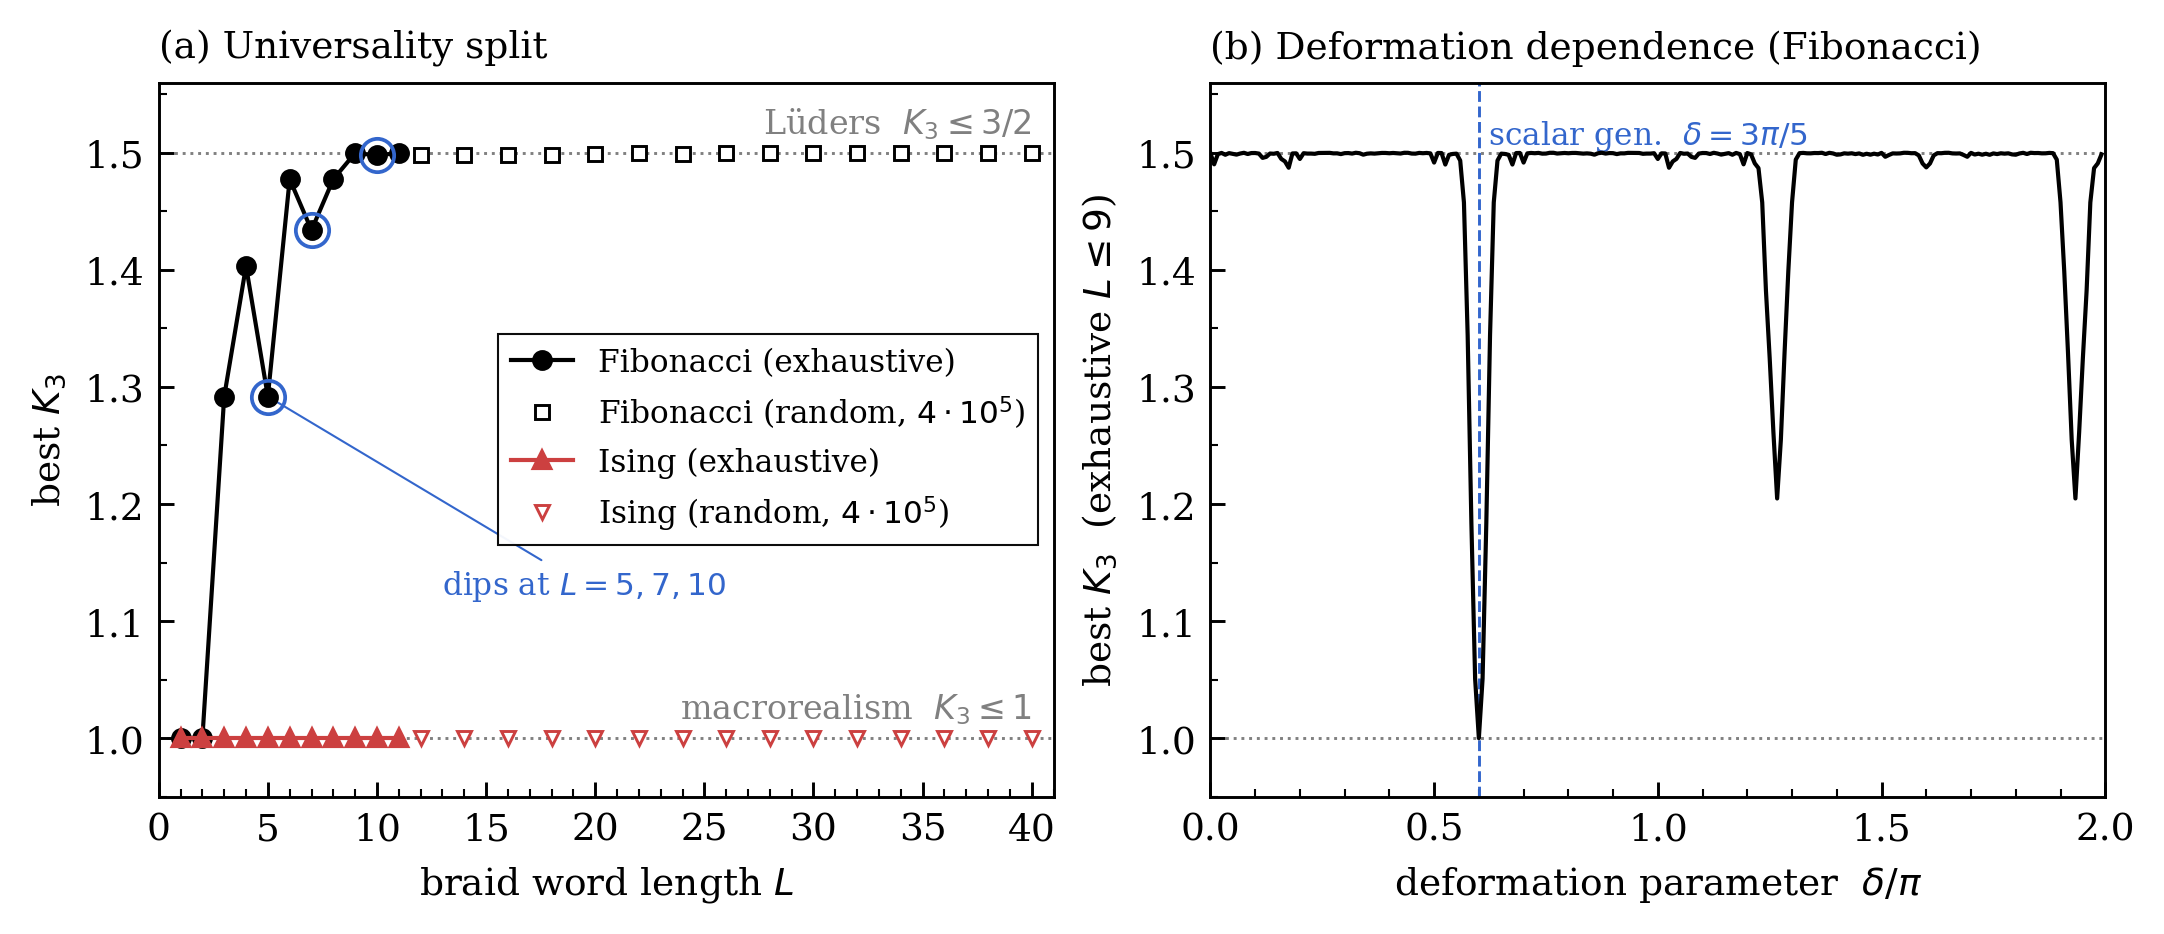
\includegraphics[width=0.95\textwidth]{lgi_letter_figure.png}
\caption{(a)~Best $K_{3}$ versus braid length $L$, $\delta=0$.
\emph{Fibonacci} (black) saturates the L\"uders bound $3/2$ to
$99.998\%$; \emph{Ising} (red) is pinned at $1.0$ for every $L$ tested
(exhaustive to $L=11$; random sampling, $4\times 10^{5}$ words per
$L$, at even $L\in\{12,14,\ldots,40\}$).
(b)~Best $K_{3}(\delta)$ envelope for Fibonacci, exhaustive
$L \leq 9$, fine sampling. The dashed line marks the algebraic
singularity $\delta = 3\pi/5$ at which $\sigma_{1}$ collapses to a
scalar (numerical scalar-deviation $3.1\times 10^{-16}$). Data:
\texttt{lgi\_results.json} and \texttt{lgi\_ising\_results.json} for
(a), \texttt{lgi\_period\_and\_purestate\_results.json} for (b); plotted
by \texttt{lgi\_letter\_figure.py}.}
\label{fig:main}
\end{figure*}

\subsection{Ising: exact $K_{3} = 1$}
\label{sec:ising}

Repeating the same search with the Ising generators gives a
qualitatively different result: $K_{3} = 1.000000$ for the best word
at \emph{every} $L \leq 11$ in the exhaustive search, and the same
for every random sample at $L \in \{12, 14, \ldots, 40\}$
(Fig.~\ref{fig:main}(a), red). The best Ising words realize
$\bigl(C(B),\, C(B^{2})\bigr) = (1,\,1)$ for the best word at each
$L \leq 10$ (the generators act as $\pm Z$ on the chosen basis), and
$(0,\,-1)$ for the $L=11$ argmax word (the generators map to $\pm
X$), both of which give $K_{3} = 1$ exactly.

This is a protocol-specific temporal counterpart of the Howard--Vala no-violation
result~\cite{HowardVala2012} for the spatial CHSH inequality: in both
cases the Ising-braiding subgroup of $\mathrm{SU}(2)$ is too small to
reach the bound. The intuition is the same: density in
$\mathrm{SU}(2)$ is, on the two-dimensional fusion space, necessary and
sufficient for saturating the L\"uders $3/2$ bound by braiding alone, just
as it is necessary for saturating the Tsirelson $2\sqrt{2}$ bound by braiding
alone; sufficiency at $d=2$ rests on the numerical sweep of the
companion study~\cite{Sayim2026SU2k}, not on an analytic proof. Ising braiding
generates only Clifford gates and is missing a non-Clifford
direction; the practical phase gate of Clarke, Sau, and
Das~Sarma~\cite{ClarkeSauDasSarma2016} supplies exactly that missing
resource in Majorana wires.

\paragraph{Cross-check against a search-space artifact.}
A clean $K_{3}=1.000000$ over the full tested range ($L\leq11$
exhaustive, even $L\in\{12,\ldots,40\}$ random) raises the natural
question whether the search has simply missed a violating word. To
rule this out, we apply the same exhaustive procedure to the
Ising generators deformed by $\delta \neq 0$ (an
algebraic generalization in which the second R-symbol is rotated to
$R_{\psi}\,e^{i\delta}$). The result is that the same code and word alphabet, searching all $4^{9}$ words of length $L = 9$ at each of $49$ grid points $\delta \in [0, 2\pi]$, recovers
$K_{3}$ values across the full range $[1.000,\,1.500]$ as $\delta$
varies, with $K_{3} = 1.500$ reached at $\delta/\pi \approx 1.167$.
A search that cannot find $K_{3} > 1$ at $\delta = 0$ is therefore
not search-limited; it is genuinely the standard Ising algebra that
forbids the violation. (We do not interpret $\delta \neq 0$ Ising as
a physical model; it is used here only as a falsification probe of
the search procedure.)

We emphasize that the $K_{3} = 1$ result is a statement about the
present two-measurement-step protocol on $\sigma$-anyon braiding
alone. A hybrid protocol that inserts an explicit non-Clifford
resource into an Ising platform---or that uses an Ising-anyon
implementation of a different gate set---could lift $K_{3}$ above $1$.
The result above is for pure braiding within the standard Ising
fusion sector.

\subsection{The scalar singularity at $\delta = 3\pi/5$}
\label{sec:singularity}

The deformation parameter $\delta$ rotates $R_{\tau}$ along the unit
circle.
At the specific point $\delta_{\star} = 3\pi/5$, the two diagonal
entries of $\sigma_{1}$ coincide:
$R_{\tau} \, e^{i\delta_{\star}}
   = e^{3\pi i/5} \, e^{3\pi i/5}
   = e^{6\pi i/5}
   = R_{1}$,
so $\sigma_{1}$ becomes a scalar times the identity. By
$\sigma_{2} = F \sigma_{1} F$ and $F^{2} = I$, $\sigma_{2}$ then
collapses to the same scalar; every braid word is a global phase, and
no $K_{3} > 1$ is achievable for any $L$. We verify this numerically:
$\|\sigma_{1}(\delta_{\star}) - e^{i\theta}\,I\| = 3.1 \times 10^{-16}$.
This is a clean, exact, machine-precision sub-result that follows
from the algebra of the F- and R-symbols alone. This collapse
threshold coincides with the intrinsic $\sigma_{1}$ rotation angle
$\delta^{\ast}(k{=}3) = \pi k/(k+2) = 3\pi/5$ of the companion
$\mathrm{SU}(2)_{k}$ analysis~\cite{Sayim2026SU2k}: both are the
relative phase $\arg(R_{1}/R_{\tau})$ of the two braid eigenvalues.

\subsection{Dependence on the deformation parameter}
\label{sec:sector-fourier}

Outside the singularity, exhaustive search with $L \leq 9$ explores
the full $\delta$ axis (Fig.~\ref{fig:main}(b)). The range of best
$K_{3}$ at fixed budget is $[1.0,\, 1.5]$, and the $K_{3} = 1$
endpoint is attained only at the algebraic singularity
$\delta^{\ast} = 3\pi/5$ itself: every nonsingular grid point violates
the inequality already at $L \leq 9$, with the weakest
envelope values ($K_{3} \approx 1.051$) at the two grid points
adjacent to the singularity ($\delta/\pi = 0.5917$ and $0.6083$).
Seeded random sampling at $\delta/\pi = 0.6083$ with longer words
raises the best value found to $K_{3} = 1.075$ at $L = 12$ and
$K_{3} = 1.148$ at $L = 24$
(\texttt{lgi\_sector\_budget\_validator.py}), a monotone recovery
consistent with a braid-budget depression that deepens continuously
toward the singular point; within the deposited budgets it remains
well short of the L\"uders bound there. The only point at which a
violation is excluded exactly is the algebraic singularity above. The
envelope is mirror-symmetric about the singular point, and hence also
about $\delta = 8\pi/5$: $K_{3,\max}(\delta) = K_{3,\max}(6\pi/5 -
\delta)$. The symmetry is exact: complex conjugation maps
$\sigma_{i}(\delta)$, and hence every word, to its counterpart at
$6\pi/5 - \delta$ up to a global phase, and the
correlator~(\ref{eq:correlator}) is invariant under $U \mapsto U^{\ast}$
because $Z$ is real, so $K_{3}(\delta;\,w) = K_{3}(6\pi/5 - \delta;\,w)$
for every word $w$; the deposited envelope satisfies it to within
$7\times 10^{-15}$, and word by word the deposited check finds at most
$2.5\times 10^{-14}$ (\texttt{lgi\_braid\_relation\_check.py}).
In particular, $\delta = 6\pi/5$ reproduces the $\delta = 0$ value
$K_{3} = 1.499762$, and the two weakest grid points $\delta/\pi =
0.5917$ and $0.6083$ are mirror images of each other.

\emph{Withdrawal of the Fourier-period analysis.} Earlier versions of
this letter reported a dominant Fourier period of the $\delta$
dependence: $k=6$ in v1.0, computed over words of exact length
$L = 9$ (it reproduces under that definition, contrary to what v1.1
and v1.2 stated), and $k=3$ in v1.1 and v1.2 for the envelope
$K_{3,\max}(\delta) = \max_{|w| \leq L} K_{3}(\delta;\,w)$,
attributed there to reshuffling of the optimal word across the sweep.
The envelope itself is not $2\pi/3$-periodic: $K_{3,\max} = 1$ only
at $\delta = 3\pi/5$, whereas $K_{3,\max}(3\pi/5 + 2\pi/3) = 1.2047$;
$k=3$ is only its largest Fourier component. An exhaustive audit of
all $349{,}524$ words with $|w| \leq 9$ on the same grid
(\texttt{lgi\_envelope\_word\_audit.py}) shows that this component is
not specific to the maximization: no single word attains the envelope
at every $\delta$, but $4{,}420$ of the $19{,}362$ words that attain
it at some grid point other than $\delta = 3\pi/5$ already have $k=3$
as the strongest harmonic of their own curve $K_{3}(\delta;\,w)$.
Most fixed-word curves are $2\pi$-periodic, but not all: $42$ of the
$924$ nonconstant curves in a random sample of $1000$ words have a
shorter period. Since, in addition, the deformed generators do not
form a braid-group representation at generic $\delta$
(Sec.~\ref{sec:setup}), we withdraw the period analysis and assign no
physical meaning to the Fourier content of the envelope.

\subsection{Initial-state independence (consistency check)}

Equation~(\ref{eq:correlator}) uses the maximally mixed initial state.
As a consistency check on that formula, we have repeated $K_{3}$ for
the optimal $L=11$ word with pure initial states $|0\rangle$,
$|1\rangle$, $|\pm\rangle$, $|\pm i\rangle$, and three Haar-random pure
states. All nine give the same value to machine precision:
\begin{center}\small
\begin{tabular}{lcc}
\toprule
initial state & $K_{3}$ & spread \\
\midrule
$|0\rangle,\ |1\rangle,\ |\pm\rangle,\ |\pm i\rangle$
              & $1.499762$ & --- \\
$3$ Haar-random pure $|\psi\rangle$
              & $1.499762$ & --- \\
\midrule
mean over pure states & $1.499762$ &
        $|\text{mean}-\text{mixed}| = 0$ \\
\bottomrule
\end{tabular}
\end{center}
This is not a special property of the L\"uders-saturating word: for
two dichotomic ($\pm1$-eigenvalue) observables $Q_{1},Q_{2}$ measured
sequentially by projective (L\"uders) measurements starting from an
arbitrary state $\rho$, the two-time correlator is exactly
$C(Q_{1},Q_{2})=\mathrm{Tr}[\rho\,\tfrac{1}{2}\{Q_{1},Q_{2}\}]$ in any
dimension. On the two-dimensional fusion space used here, $Q_{1}=Z$
and $Q_{2}=UZU^{\dagger}$ are \emph{both} traceless Hermitian
operators with eigenvalues $\pm1$ for \emph{every} unitary $U$
(Bloch-vector operators on a qubit), and any two such operators
have an anticommutator proportional to the identity,
$\{Q_{1},Q_{2}\}\propto I$ -- a generic $d=2$ Pauli-algebra identity,
not a property singled out by the L\"uders-saturating word.
Consequently $C(U)$, and hence $K_{3}$, is exactly independent of
$\rho$ for every braid word $U$, optimal or not. The measurement
above is therefore a consistency check on
Eq.~(\ref{eq:correlator}) rather than an independent finding: it
confirms that the deposited code correctly implements the trace
formula, and pre-empts a natural reviewer concern that the
mixed-state convention might mask a more nuanced state dependence.

\section{Discussion}
\label{sec:discussion}

\paragraph{What the universality split says.}
The pair (Fibonacci, Ising) is the natural minimal test bed for
universality-driven phenomena in non-Abelian anyon platforms.
Howard and Vala~\cite{HowardVala2012} established that Ising braiding
alone cannot violate the spatial CHSH inequality (any violation
requires a non-stabilizer operation---gates and measurements
together); Clarke, Sau, and
Das~Sarma~\cite{ClarkeSauDasSarma2016} supply a practical phase gate
providing exactly that missing resource in Majorana wires. The
universal Fibonacci model, by contrast, saturates the bound by
density~\cite{NayakSimonStern2008}, Brennen \emph{et al.}~\cite{Brennen2009}
constructing explicit (sub-Tsirelson) CHSH-violating settings. The present results
show that the same split holds for the \emph{temporal} inequality:
Fibonacci saturates the L\"uders bound to $99.998\%$ while Ising is
pinned at $1.0$ on the two-dimensional fusion space. In a single
sentence: under projective L\"uders measurement from a maximally mixed
state on the two-dimensional fusion space, universality is a property
that allows a non-Abelian anyon braid to saturate both the spatial
and the temporal projective-quantum bounds.

\paragraph{What it does not say.}
The Fibonacci L\"uders saturation is not, by itself, evidence for a
nonclassical \emph{topological} mechanism beyond what the modular
tensor category already prescribes. Fibonacci density in
$\mathrm{SU}(2)$ guarantees that any unitary---including the one
realizing the L\"uders-saturating product---can be approximated by a
braid word; the role of topology here is to provide that universal
gate set, not to add an additional nonclassical resource. The
Leggett--Garg saturation is a TQFT-consistency demonstration, in the
same sense in which the spatial CHSH saturation is a TQFT-consistency
demonstration. The interest of the result lies in (i) closing the
non-Abelian Bell/Leggett--Garg literature gap, (ii) the sharpness of the
Fibonacci/Ising split, and (iii) the algebraic scalar singularity at
$\delta = 3\pi/5$. $K_{3}$ is computed here for
projective L\"uders measurement of $Q$ at every time step and a
maximally mixed (or, equivalently by Sec.~\ref{sec:results}, any
pure) initial state; its behavior under weak or nonprojective
measurement protocols is not addressed and is left open.

\paragraph{Relation to G\'omez-Ruiz~\textit{et~al.}~2018.}
G\'omez-Ruiz \emph{et al.}~\cite{GomezRuiz2018} test the three-time
LGI in the form $K_{i,j}(t) = 2\,C_{i,j}(t) - C_{i,j}(2t) \leq 1$ on
Dirac qubits formed from edge Majorana modes of the Kitaev chain.
That system is abelian; the test serves as a probe of the topological
phase transition. Their maximum reported violation $K_{\rm Max}(\mu)$
reaches $\approx 1.5$ across a chemical-potential sweep but is not
analyzed as a saturation distance to the L\"uders bound. The present
work tests $K_{3}$ on the non-Abelian fusion-channel qubit of three
$\tau$ anyons; the Fibonacci-Ising universality split is the central
comparison; and the saturation is reported as a $3.6 \times 10^{-5}$
gap to the L\"uders bound (i.e.\ $99.998\%$) obtained by braid-word
optimization, rather than as a transition diagnostic. Both works
belong to the genre ``Leggett--Garg on a topological system''; they
are methodologically and physically distinct sub-cases.
G\'omez-Ruiz \emph{et al.}\ nonetheless serves as the relevant
reference point for this line of work. Their setting is abelian, and
braiding in such Majorana realizations is confined to the Clifford
group (a property of the platform, not a claim made in their work);
it is the one published precedent against
which any non-Abelian, universal-braiding LGI test---including the
companion $\mathrm{SU}(2)_k$ study discussed below---must be
distinguished.

\paragraph{What an experiment would look like.}
A direct test requires (i) a platform supporting non-Abelian
braiding---present candidates are filling-fraction $\nu = 12/5$ for
Fibonacci~\cite{NayakSimonStern2008} and quantum-processor
implementations of Fibonacci string-nets~\cite{Xu2024,Minev2025};
(ii) projective measurement of the fusion channel of an anyon
pair~\cite{Bonderson2008}; (iii) the ability to apply a deterministic
braid word between measurements. The Howard--Vala no-violation result
predicts that for this Ising braid representation, under the present
sequential $B_3$ L\"uders protocol on the two-dimensional fusion space,
the $K_{3}$ would be pinned at $1$ even in the absence of decoherence;
the digital topological realizations of
Refs.~\cite{Andersen2023,Iqbal2024} implement a different, spatial
setting.
The robustness of $K_{3}$ to depolarizing noise on the platform
benchmark of~\cite{Andersen2023} would have to be analyzed
separately, following the decoherence-threshold framework
of~\cite{Emary2013}. An experimental test would additionally have to address the clumsiness loophole---that a violation could be caused by the measurements disturbing the system~\cite{WildeMizel2012,EmaryLambertNori2014}.

\section{Open questions}
\label{sec:open}

Three natural extensions are immediate but outside the scope of this
note:
\begin{enumerate}
\item[\textbf{O1.}] $K_{n}$ for $n > 3$. For $n$ equally spaced
projective measurements the L\"uders bound is
$K_{n}^{\max} = n\cos(\pi/n)$~\cite{EmaryLambertNori2014}, approaching
the algebraic limit $K_{n} \to n$ as $n \to \infty$. Whether
Fibonacci braiding saturates this moving bound at each $n$ is
untested here; a multi-time Leggett--Garg test with $n=4,5,\ldots$ is
a one-day extension of the present setup.
\item[\textbf{O2.}] Structural origin of the nonmonotonicity dips.
The proximate cause of the dips at $L = 5, 7, 10$ is geometric: at
those lengths the best reachable braid word lands farther from the
$K_{3}$-optimal rotation than at neighboring lengths, so the
per-length maximum drops. Whether this reachability pattern is
governed at a deeper level by the divisibility structure of the
central element $(\sigma_{1}\sigma_{2})^{3}$ of $B_{3}$ is left open;
a systematic correlation of dip-position with the algebra would be a
sharper version of ``best at length $L$'' than the running maximum.
\item[\textbf{O3.}] Representation dependence of the temporal bound.
Sorella~\cite{Sorella2023} has shown that in dimensions higher than
two the Bell operators admit unitarily inequivalent representations,
so that the \emph{attained} CHSH violation is representation-dependent,
with Tsirelson's bound as the invariant maximum. The
temporal counterpart---whether the L\"uders bound $3/2$ is
representation-dependent in $\dim > 2$ fusion spaces---is open. Our
setup is fixed at $\dim = 2$; a $\dim > 2$ extension would address
this directly. This question is supplemented by a companion work on
the $\mathrm{SU}(2)_k$ family across braid-representation
dimension~\cite{Sayim2026SU2k}.
\end{enumerate}

\section*{Notation}
\noindent Symbols used in this paper.
\begin{ruledtabular}
\begin{tabular}{ll}
Symbol & Meaning \\
\hline
$L$ & \parbox[t]{0.72\columnwidth}{braid-word length} \\
$\sigma_{1},\sigma_{2}$ & \parbox[t]{0.72\columnwidth}{generators (braid generators at $\delta = 0$), $\sigma_{1} = \mathrm{diag}(R_{1},\,R_{\tau}\,e^{i\delta})$, $\sigma_{2} = F\,\sigma_{1}\,F$} \\
$F$, $R_{1}$, $R_{\tau}$ & \parbox[t]{0.72\columnwidth}{standard Fibonacci $F$- and $R$-symbols, $R_{1} = e^{-4\pi i/5}$, $R_{\tau} = e^{+3\pi i/5}$} \\
$\delta$ & \parbox[t]{0.72\columnwidth}{algebraic phase-deformation parameter of the generators; $\delta = 0$ recovers the standard Fibonacci theory} \\
$C(B)$, $C(B^{2})$ & \parbox[t]{0.72\columnwidth}{two-time correlators of L\"uders measurements of $Q = \sigma_{z}$ separated by the braid $B$ and by $B^{2}$} \\
$K_{3}$ & \parbox[t]{0.72\columnwidth}{three-time Leggett--Garg combination, $K_{3} = 2\,C(B) - C(B^{2})$} \\
\end{tabular}
\end{ruledtabular}

\section*{Data and Code Availability}

Paper, figures, and data are released under the Creative Commons
Attribution 4.0 International (CC~BY~4.0) license; the deposited source
code is released under the Apache License 2.0 (\texttt{LICENSE} and
\texttt{LICENSE-CODE} in the record;
\url{https://creativecommons.org/licenses/by/4.0/}). All code and result
files are deposited with this record~\cite{Sayim2026LGIdata}.
Reproduction is deterministic with the random seeds
\texttt{20260524} (Fibonacci main),
\texttt{20260525} (Ising, period scan, and pure-state robustness),
\texttt{20260723} (sector budget validator,
\texttt{lgi\_sector\_budget\_validator.py}), and \texttt{20260928}
(envelope word audit, \texttt{lgi\_envelope\_word\_audit.py}). The
braid-relation and mirror-symmetry checks of Secs.~\ref{sec:setup}
and~\ref{sec:sector-fourier} are reproduced by
\texttt{lgi\_braid\_relation\_check.py}. All
computations use only \texttt{numpy} and \texttt{matplotlib}.
Sanity checks at the head of \texttt{lgi\_fibonacci.py} and
\texttt{lgi\_ising.py} (unitarity, Yang--Baxter, $(\sigma_1\sigma_2)^3$
scalar, all at $\delta = 0$) must pass at machine precision; if they
do not, the generator conventions have been altered.

\section*{Use of AI tools}

In the research, processing, and writing of this paper and its results I worked together with generative AI tools, in practice a system of multiple coordinated AI instances that I set up and orchestrate (large language models, mainly Claude, by Anthropic, inside Claude Code). At their current context sizes I found it far more effective to work with several specialized instances, each with its own role and its own harness of rules and parameters that I designed and refined through feedback, than to load a single instance with all of the material; for my workflow that would have been inefficient, though this depends on the individual implementation. I lead this collaboration: I choose the research directions, set the goals, and make the final decisions in open exchange with the AI, learning actively as the work proceeds. The AI carries out the drafting, including the mathematical and technical parts, the numerical computation, and the literature search, under my direction. The AI works autonomously only task by task, within the structure I develop through feedback: it completes a task, and at open questions that need me it stops until the point is settled before the next step. Along the way I witness and take many of the decisions that shape the path, and it is common for me to spot things that need improvement. The work spans many separate runs, and a single simulation or build task alone can take up to an hour, so it could not happen all together in one autonomous run; and had I let the AI do all of it together alone, even if it is possible, it would no longer be my work but the AI's.

I run multiple verifications at the different stages of the work and one before release, including cross-checks with an unrelated AI model from a different company, and all references are checked against the original sources. In the end what matters are human eyes, a principle that is itself written into the parameters of my system: I reach out to experts after publishing for review and feedback, so I learn what is solid and what must be corrected or falsified. My scripts for reproduction and review are released with this record. These tools are not authors; I am the author, and I take full responsibility for all scientific content and decisions leading to these results and their publication.

\section*{Acknowledgments}

This research received no specific grant from any funding agency in the
public, commercial, or not-for-profit sectors. The author declares no
competing interests.

\begin{thebibliography}{99}

\bibitem{LeggettGarg1985}
A.~J.~Leggett and A.~Garg,
\emph{Quantum mechanics versus macroscopic realism: Is the flux there when nobody looks?}
Phys.\ Rev.\ Lett.\ \textbf{54}, 857 (1985).

\bibitem{Budroni2014}
C.~Budroni and C.~Emary,
\emph{Temporal quantum correlations and Leggett-Garg inequalities in multi-level systems},
Phys.\ Rev.\ Lett.\ \textbf{113}, 050401 (2014);
\href{https://arxiv.org/abs/1309.3678}{arXiv:1309.3678}.

\bibitem{EmaryLambertNori2014}
C.~Emary, N.~Lambert, and F.~Nori,
\emph{Leggett-Garg inequalities},
Rep.\ Prog.\ Phys.\ \textbf{77}, 016001 (2014);
\href{https://arxiv.org/abs/1304.5133}{arXiv:1304.5133}.

\bibitem{Fritz2010}
T.~Fritz,
\emph{Quantum correlations in the temporal CHSH scenario},
New J.\ Phys.\ \textbf{12}, 083055 (2010);
\href{https://arxiv.org/abs/1005.3421}{arXiv:1005.3421}.

\bibitem{Emary2013}
C.~Emary,
\emph{Decoherence and maximal violations of the Leggett-Garg inequality},
Phys.\ Rev.\ A \textbf{87}, 032106 (2013);
\href{https://arxiv.org/abs/1212.3865}{arXiv:1212.3865}.

\bibitem{KoflerBrukner2008}
J.~Kofler and \v{C}.~Brukner,
\emph{The conditions for quantum violation of macroscopic realism},
Phys.\ Rev.\ Lett.\ \textbf{101}, 090403 (2008);
\href{https://arxiv.org/abs/0706.0668}{arXiv:0706.0668}.

\bibitem{NayakSimonStern2008}
C.~Nayak, S.~H.~Simon, A.~Stern, M.~Freedman, and S.~Das~Sarma,
\emph{Non-Abelian anyons and topological quantum computation},
Rev.\ Mod.\ Phys.\ \textbf{80}, 1083 (2008).

\bibitem{Bonderson2008}
P.~Bonderson, M.~Freedman, and C.~Nayak,
\emph{Measurement-only topological quantum computation},
Phys.\ Rev.\ Lett.\ \textbf{101}, 010501 (2008).

\bibitem{ClarkeSauDasSarma2016}
D.~J.~Clarke, J.~D.~Sau, and S.~Das~Sarma,
\emph{A practical phase gate for producing Bell violations in Majorana wires},
Phys.\ Rev.\ X \textbf{6}, 021005 (2016);
\href{https://arxiv.org/abs/1510.00007}{arXiv:1510.00007}.

\bibitem{HowardVala2012}
M.~Howard and J.~Vala,
\emph{Nonlocality as a benchmark for universal quantum computation in Ising anyon topological quantum computers},
Phys.\ Rev.\ A \textbf{85}, 022304 (2012);
\href{https://arxiv.org/abs/1112.1516}{arXiv:1112.1516}.

\bibitem{Brennen2009}
G.~K.~Brennen, S.~Iblisdir, J.~K.~Pachos, and J.~K.~Slingerland,
\emph{Non-locality of non-Abelian anyons},
New J.\ Phys.\ \textbf{11}, 103023 (2009);
\href{https://arxiv.org/abs/0810.4319}{arXiv:0810.4319}.

\bibitem{GomezRuiz2018}
F.~J.~G\'omez-Ruiz, J.~J.~Mendoza-Arenas, F.~J.~Rodr\'iguez,
C.~Tejedor, and L.~Quiroga,
\emph{Universal two-time correlations, out-of-time-ordered
correlators and Leggett-Garg inequality violation by edge Majorana
fermion qubits},
Phys.\ Rev.\ B \textbf{97}, 235134 (2018);
\href{https://arxiv.org/abs/1802.10522}{arXiv:1802.10522}.

\bibitem{Sorella2023}
S.~P.~Sorella,
\emph{On the representations of Bell's operators in Quantum Mechanics},
Found.\ Phys.\ \textbf{53}, 59 (2023);
\href{https://arxiv.org/abs/2304.05696}{arXiv:2304.05696}.

\bibitem{Andersen2023}
T.~I.~Andersen \emph{et al.} (Google Quantum AI and Collaborators),
\emph{Non-Abelian braiding of graph vertices in a superconducting processor},
Nature \textbf{618}, 264 (2023);
\href{https://arxiv.org/abs/2210.10255}{arXiv:2210.10255}.

\bibitem{Iqbal2024}
M.~Iqbal, N.~Tantivasadakarn, R.~Verresen, S.~L.~Campbell,
J.~M.~Dreiling, C.~Figgatt, J.~P.~Gaebler, J.~Johansen, M.~Mills,
S.~A.~Moses, J.~M.~Pino, A.~Ransford, M.~Rowe, P.~Siegfried, R.~P.~Stutz,
M.~Foss-Feig, A.~Vishwanath, and H.~Dreyer,
\emph{Non-Abelian topological order and anyons on a trapped-ion processor},
Nature \textbf{626}, 505 (2024).

\bibitem{Xu2024}
S.~Xu, Z.-Z.~Sun, K.~Wang, H.~Li, Z.~Zhu, H.~Dong, J.~Deng, X.~Zhang,
J.~Chen, Y.~Wu, C.~Zhang, F.~Jin, X.~Zhu, Y.~Gao, A.~Zhang, N.~Wang,
Y.~Zou, Z.~Tan, F.~Shen, J.~Zhong, Z.~Bao, W.~Li, W.~Jiang, L.-W.~Yu,
Z.~Song, P.~Zhang, L.~Xiang, Q.~Guo, Z.~Wang, C.~Song, H.~Wang,
and D.-L.~Deng,
\emph{Non-Abelian braiding of Fibonacci anyons with a superconducting processor},
Nat.\ Phys.\ \textbf{20}, 1469 (2024);
\href{https://arxiv.org/abs/2404.00091}{arXiv:2404.00091}.

\bibitem{Minev2025}
Z.~K.~Minev, K.~Najafi, S.~Majumder, J.~Wang, A.~Stern,
E.-A.~Kim, C.-M.~Jian, and G.~Zhu,
\emph{Realizing string-net condensation: Fibonacci anyon braiding
for universal gates and sampling chromatic polynomials},
Nat.\ Commun.\ \textbf{16}, 6225 (2025);
\href{https://arxiv.org/abs/2406.12820}{arXiv:2406.12820}.

\bibitem{Sayim2026LGIdata}
B.~Y.~Sayim,
\emph{Code and data for: Leggett--Garg saturation and structural
signatures in Fibonacci-anyon braiding},
Zenodo (2026);
\href{https://doi.org/10.5281/zenodo.20372744}{doi:10.5281/zenodo.20372744}.

\bibitem{Sayim2026SU2k}
B.~Y.~Sayim,
\emph{A dichotomous Leggett--Garg witness for braid-representation
density in $\mathrm{SU}(2)_k$: exact at $d=2$, dimension-limited at
$d \ge 3$},
Zenodo preprint (2026);
\href{https://doi.org/10.5281/zenodo.20531124}{doi:10.5281/zenodo.20531124}.

\bibitem{WildeMizel2012}
M.~M.~Wilde and A.~Mizel,
\emph{Addressing the clumsiness loophole in a Leggett-Garg test of macrorealism},
Found.\ Phys.\ \textbf{42}, 256 (2012);
\href{https://arxiv.org/abs/1001.1777}{arXiv:1001.1777}.

\end{thebibliography}

\end{document}
